\chapter{Time Is Valuable}

These notes follow Jim Rohn's lecture as preserved in a curated LazyingArt LLC playlist rather than a clean institutional course. The title speaks of time, but the lecture begins somewhere more primitive: with self-interest, survival, success, and the claim that life does not hand us results merely because we need them. Only after that first law has been stated and driven through several examples does the talk widen into service, leadership, personal development, patience, and finally a concrete procedure for solving problems on paper. The mathematics here is therefore structural rather than quantitative. It is a way of preserving the lecture's sequence and its logic of qualification.

\paragraph{Heuristic status.}
No validated blackboard frames survive for this lecture, so every displayed formula and diagram below is transcript-backed or a cautious reconstruction of the spoken argument. These displays are not formal economics or psychology. They are deliberate summaries of a lecture whose central claims are procedural.

\section{Enlightened Self-Interest and the Law of Deserving}

The lecture opens in seminar mode. Rohn tells the audience he wants to get busy on the first subjects of the day, asks them to jot things down, and names the first subject immediately: enlightened self-interest. The tone matters. We are not entering a detached theory. We are being led, step by step, through a sequence of notes the speaker regards as life-changing.

The first statement is simple enough:
\begin{equation}
\text{self-interest} \rightarrow \{\text{survival},\text{success}\}.
\end{equation}
Our first interest is to survive; our second is to succeed. Rohn does not deny this. The entire lecture would collapse if it began by pretending that self-interest were shameful or unreal.

The lecture's first refinement is that the self-interest must be educated:
\begin{equation}
S_{\mathrm{enl}}=\text{self-interest constrained so that everybody wins and no one loses}.
\end{equation}
This is not a rigorous game-theoretic formula, and it should not be hardened into one. It is a moral and practical gloss. Self-interest becomes enlightened when it learns sequence, law, and consequence.

A short stretch of transcript is garbled exactly when Rohn makes the next transition, but the safe content is clear. He is moving from self-interest to a stronger claim about how the world is structured. In his language, life and God do not give us things merely because we need them. They give us what we deserve.

\begin{definition}
In the lecture's operational sense, deserving does not mean moral superiority. It means that some qualifying action has begun and has been sustained far enough that a result is now due.
\end{definition}

That yields the chapter's governing maxim:
\begin{equation}
\text{we get not what we need, but what we deserve}.
\end{equation}

The lecture immediately narrows the meaning further. There are moral and spiritual laws, Rohn says, but here he wants the more basic structure: if we wish to reap, we must plant. The point is that deserving is attached to action and order, not to inward wishing alone. That is what makes the rest of the lecture mathematically compressible.

\section{Plant, Knock, Search, Ask}

Once the law of deserving is on the table, Rohn does not leave it abstract. He drives it through a chain of parallel examples. The repetition is essential. Each example says the same thing again, but with a little more force and a little more range.

\begin{align}
\text{need} &\not\Rightarrow \text{harvest}, &
\text{planting} &\Rightarrow \text{deserved reaping}, \\
\text{continual knocking} &\rightarrow \text{open doors}, &
\text{searching} &\rightarrow \text{finding}, \\
\text{asking} &\rightarrow \text{qualification for answers}. &&
\end{align}

The agricultural form comes first because it is the clearest. We do not reap in the fall because we need the crop. We reap because planting has been done. In Rohn's own phrase, reaping is reserved for the planters. This is stronger than a piece of encouragement. It is the lecture's model of lawful consequence.

The same structure is then carried into opportunity. We do not find open doors because we need opportunity. We find them because we have kept knocking. The promise is attached to repeated action, not to exposed lack. From there the extension is immediate. Finding is reserved for the searchers; answers belong to those who ask.

\begin{figure}[t]
\centering
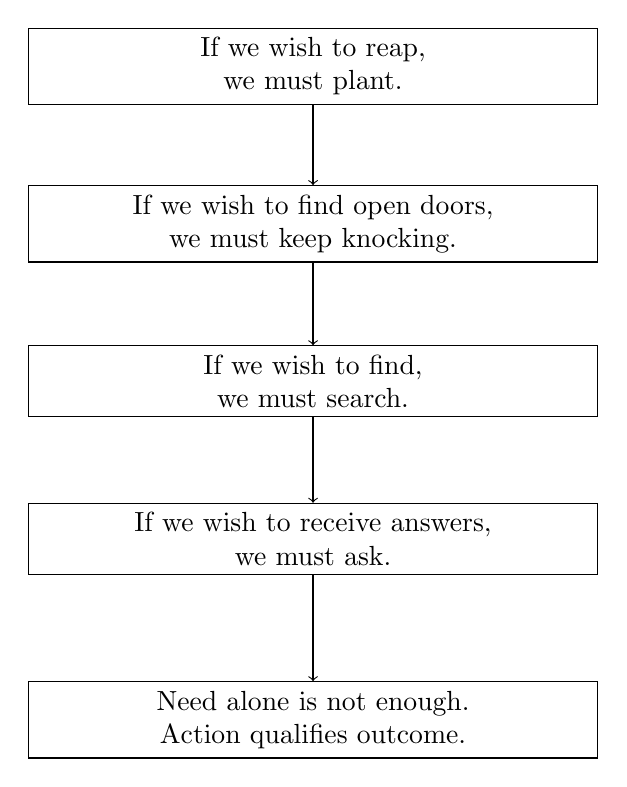
\begin{tikzpicture}[x=1cm,y=1cm]
\node[draw,align=center,text width=7cm] (a) at (0,0) {If we wish to reap,\\we must plant.};
\node[draw,align=center,text width=7cm] (b) at (0,-2.0) {If we wish to find open doors,\\we must keep knocking.};
\node[draw,align=center,text width=7cm] (c) at (0,-4.0) {If we wish to find,\\we must search.};
\node[draw,align=center,text width=7cm] (d) at (0,-6.0) {If we wish to receive answers,\\we must ask.};
\node[draw,align=center,text width=7cm] (e) at (0,-8.3) {Need alone is not enough.\\Action qualifies outcome.};
\draw[->] (a) -- (b);
\draw[->] (b) -- (c);
\draw[->] (c) -- (d);
\draw[->] (d) -- (e);
\end{tikzpicture}
\caption{A transcript-backed deserve-logic ladder. The lecture's four maxims are parallel cases of one rule: outcomes are attached to qualifying action.}
\end{figure}

Rohn then pauses to apply the same logic to the room he is speaking to. The audience has come searching. They got on airplanes, into automobiles, and arrived in a receptive state. Therefore they are now in position to receive plans, answers, and imagination. The seminar is not treated as a mystical interruption. It is treated as the continuation of the search process.

One of the lecture's best local lines belongs here: rarely does a good idea interrupt us. If we wish to find a good idea, we must go looking. Church, class, seminary, library, books---all are named as places of deliberate search.

\subsection{Question \& Answer}

The lecture naturally raises a local objection here. If harvest, opportunity, and answers are all deeply needed, why are they not granted simply because they are needed?

Rohn's answer is that need indicates lack, but not yet qualification. In compact form,
\begin{equation}
N \not\Rightarrow R, \qquad N + Q \Rightarrow D \Rightarrow R,
\end{equation}
where \(N\) denotes need, \(Q\) the qualifying process, \(D\) deserving, and \(R\) the result. Need may awaken the search, but it is not identical with the search. That is why the lecture keeps returning to active verbs: plant, knock, search, ask.

\section{Need, Seed, and the Process of Deserving}

The lecture now pivots from maxim to mechanism. This is where the notes must not become too polished and abstract, because the concrete examples are doing real work. Rohn wants to show what the law of deserving looks like in ordinary life.

A careful reconstruction of the central idea is
\begin{equation}
\text{deserving}=\text{qualifying action sustained over time}.
\end{equation}

The welfare example should be read exactly in that spirit. Rohn is not claiming that painting a door and a fence is equivalent in market price to a welfare check. He is saying something narrower and, within the lecture, more important: a small qualifying act can begin a new process.

\paragraph{Worked example: the beginning of deserving.}
Let \(D_n\) denote the current level of qualification and let \(A_n\) denote the \(n\)-th qualifying act. Then the lecture's example may be organized as
\begin{align}
D_0 &= \text{need alone}, &
D_0 &\not\Rightarrow \$450, \\
A_1 &= \text{paint the door and the fence}, &
D_1 &= D_0 + A_1, \\
A_2 &= \text{clear the weeds and cultivate the garden}, &
D_2 &= D_1 + A_2.
\end{align}
The dollars remain assistance; the point is not market valuation but process. The lecture's operative picture is
\begin{equation}
D_{n+1}=D_n + A_{n+1},
\end{equation}
so that step by step a new life emerges. Rohn says exactly this: one begins learning the process of deserving, not merely needing.

The same logic is immediately repeated at home. A child says, ``I need ten dollars.'' Rohn's answer is that such language does not open the vault. The better question is: how could I earn ten dollars?
\begin{equation}
\text{need} \not\Rightarrow \$10, \qquad \text{earn}(\$10) \Rightarrow \text{vault opens}.
\end{equation}

This is then broadened once more by the field and the marketplace. One cannot walk to the field and declare a need for crops while bringing no seed. One cannot carry bare need into the marketplace and expect the resources of the world to flow in response. Rohn deliberately sharpens the contrast:
\begin{equation}
\text{take your seed to the marketplace, not your need}.
\end{equation}

What does the marketplace care about? The lecture answers in a list:
\begin{equation}
\text{marketplace interest}
=
\{\text{seed},\text{willingness},\text{discipline},\text{eagerness},\text{vitality},\text{work ethic}\}.
\end{equation}

Need may be psychologically urgent, but it is not yet value. Seed, willingness, and work are the beginning of value. That is why Rohn pairs the field with the bank vault and the marketplace: each rejects mere need and responds to qualifying action.

He also inserts a theological version of the same law. If we move toward God, God moves toward us. Here again the form is the same: the move must begin somewhere. Whether we speak of crops, money, opportunity, or spiritual meeting, the lecture keeps asking for the first movement.

\subsection{Question \& Answer}

The better question now is not ``How do I get what I need?'' but ``What process should I begin engaging in to deserve good health, good relationships, prosperity, and enterprise?''

The answer is deliberately modest. One does not begin with the finished life. One begins with the first disciplined act:
\begin{equation}
\text{state of need} \rightarrow \text{first disciplined act} \rightarrow \text{process of deserving}.
\end{equation}

That is why the lecture prefers seed to need, earning to requesting, and cultivation to complaint. The key word is \emph{begin}. Deserving is not first a reward sitting at the end of the road. It is the road itself, entered by small actions that can be repeated.

\section{Giving, Service, Greatness, and Faithfulness in Small Things}

At this point the lecture returns explicitly to enlightened self-interest. The desire to receive is not condemned. It is named as self-interest. But self-interest becomes enlightened only when it understands sequence:
\begin{align}
\text{if you wish to receive, you must give}, \\
\text{receiving is reserved for those who give}, \\
\text{giving} \rightarrow \text{receiving process begins}.
\end{align}

This is Rohn's explanation of the saying that it is better to give than to receive. He is not merely praising generosity as a beautiful sentiment. He is identifying process order. At the beginning of the cycle, giving is to receiving what planting is to harvest.

A corrupt stretch of transcript interrupts the middle of this discussion, but the secure surrounding point is strong. Rohn says that some forms of receiving cannot be purchased with money. Later gratitude from someone whose life was changed by a seminar is not a commodity. It must be earned. That line deepens the argument: giving starts the receiving process not only for money, but for significance.

From there the lecture expands. How do we become great?
\begin{equation}
\text{service to many} \rightarrow \text{greatness}.
\end{equation}

Rohn takes care to stage the weaker alternatives first. Self-care has a reward, but it is limited. Self-preservation has a place, but it does not generate abundance. If we want to move from mere self-defense to greatness, then we must help solve other people's problems and help find answers for them.

The next escalation is from greatness in general to leadership and stewardship in particular. How do we become ruler over many? How do we preside over riches, manage large organizations, or speak to vast audiences? The answer is surprisingly small:
\begin{align}
\text{faithful with little} &\rightarrow \text{qualified for much}, \\
\text{discipline with small amounts} &\rightarrow \text{qualification for riches and stewardship}, \\
\text{few listeners treated faithfully} &\rightarrow \text{qualification to speak to many}.
\end{align}

This is one of the lecture's most important pieces of structure. The small paycheck, the few people, and the small audience are not accidents at the edge of the real story. They are the real story at its beginning. If a person does not know where the small amount goes, that disorder disqualifies him from stewardship over the larger amount. If a speaker is indifferent to the few, he is not yet being shaped for the many.

Rohn then places himself under the same law. He did not begin before great crowds. He began with just a few, trying in awkward ways to translate what had happened to him. This autobiographical moment is not ornamental. It verifies the principle. Qualification does not descend whole. It starts in fidelity to the limited scene presently before us.

\section{Personal Development as Refinement: Change, Library, Ideas, and Plans}

Only after the deserve-logic has been driven through work, service, and stewardship does the lecture broaden into personal development in a more general sense. The first note here is not accumulation but refinement. We are to give ourselves a chance to change, revise what we once held fixed, and allow a new direction to appear.

The lecture almost states the transition as a rule:
\begin{equation}
\text{re-evaluation} \rightarrow \text{new door}.
\end{equation}

This is not indecision elevated into principle. It is the claim that stubborn attachment to an earlier version of ourselves can prevent later discovery. To refine philosophy is to make room for doors not previously visible.

The library then appears as a physical sign of seriousness. Let the library testify, Rohn says, to our dedicated interest in accelerated personal development. Read what must be read, hear what must be heard, watch what must be seen. The seminar itself is described as a stopping station and a catalyst. We are to sit, listen, ponder, take notes, and work, so that refinement has begun before we even return home.

A noisy stretch of transcript follows, but its recoverable meaning is clear enough to preserve. Even a reaction of disagreement can be useful if it proves that the mind is awake. What matters is alertness, receptivity, and the ability to take the best of what comes and turn it into benefit. This belongs here because it explains why the seminar can function as a catalyst rather than as passive entertainment.

The lecture then condenses the next stage into a compact success formula:
\begin{equation}
\text{good ideas} + \text{good plans} + \text{time-handling} \rightarrow \text{steps to success}.
\end{equation}

Rohn is especially insistent that ideas do not come singly:
\begin{equation}
\text{one good idea} \rightarrow \text{next idea} \rightarrow \text{further acceleration}.
\end{equation}

That is why he speaks in multiplicative language: two times, three times, five times more than we previously thought possible. The lecture is not claiming a law of exact numerical growth. It is claiming that one idea changes our access to later ideas.

The plans he names are concrete and deliberately varied: a health plan, a family plan, a marriage plan, a plan for how to use the day, a plan for meeting the right people over the right amount of time, and a game plan for lifestyle. A life left undesigned tends to drift. The lecture therefore asks us to treat planning not as decoration but as one of the actual forms of self-development.

\section{Time, Patience, and the Rule That Most Will}

Now the lecture arrives directly at its title theme. Everything up to this point has required time, and the failure to understand time produces a distinctive kind of discouragement. We want growth, but we want it without season.

\begin{equation}
\text{time} + \text{patience} \rightarrow \text{growth, learning, and change}.
\end{equation}

Rohn first returns to the crop. One cannot plant the seed and then dig around every few days asking where it is. Some people plant in the spring and leave in the summer; they do not stay long enough for the season to do its work. This is the agricultural version of impatience.

The lecture then extends the same structure outward. Projects need time. People need time. Families need time. Independent personalities especially need time. The comic metaphor of herding cats makes the point vividly: coordination among free persons is difficult, and patience is not a sentimental extra but a working requirement.

The next turn is inward. We must have patience with ourselves. Learning, change, and refinement do not occur at identical speeds for all people. Rohn uses the example of learning to tie one's shoes. The image is elementary on purpose. It reminds us that all growth has this form: repetition, failure, adjustment, and gradual mastery. The adult version is no different in structure.

The social extension of patience is then given in one of the lecture's strongest general rules:
\begin{equation}
\text{usually enough good people} \rightarrow \text{social stability}.
\end{equation}

Rohn phrases this repeatedly as ``most will'' or ``enough will.'' He does not claim that every citizen, senator, teenager, employer, or official will do the right thing. He claims something weaker and more practical: enough people usually will, and that is how a civilized society remains livable.

The Sodom-and-Gomorrah story serves as an explicit exception. Abraham keeps lowering the threshold---fifty, forty, thirty, ten---and still cannot find enough righteous people. That is the exceptional failure case. It is included precisely to clarify the general rule. Ordinarily, enough people hold the structure together.

We should not formalize this beyond the lecture. ``Most will'' is not a probability theorem. It is a confidence condition for practical patience. It explains why patient effort in family, business, and society is usually rational.

\section{Thinking on Paper: A Procedure for Solving Problems}

The lecture's final major pivot is announced cleanly: next under personal development is learning to solve problems. After long arcs about deserving, service, and patience, the talk becomes procedural. This is the clearest algorithm in the lecture.

The first move is to relocate the problem:
\begin{equation}
\text{problem in head} \rightarrow \text{problem on paper} \rightarrow \text{sortable object of thought}.
\end{equation}

The reason is immediate. The mind is busy. It mixes together emotion, haste, memory, fear, and fragments of explanation. Once the problem is written down, we can ask a more precise question: have we described all of it? If not, we are not yet ready to prescribe anything for it.

\subsection{Question \& Answer}

The natural question is this: how do we solve a problem when the mind is too busy to sort it out?

Rohn's answer is to think on paper. A page is divided in two. On the left we describe the problem; on the right we write answers and solutions. This is not a literary exercise. It is a device for analysis.

\begin{figure}[t]
\centering
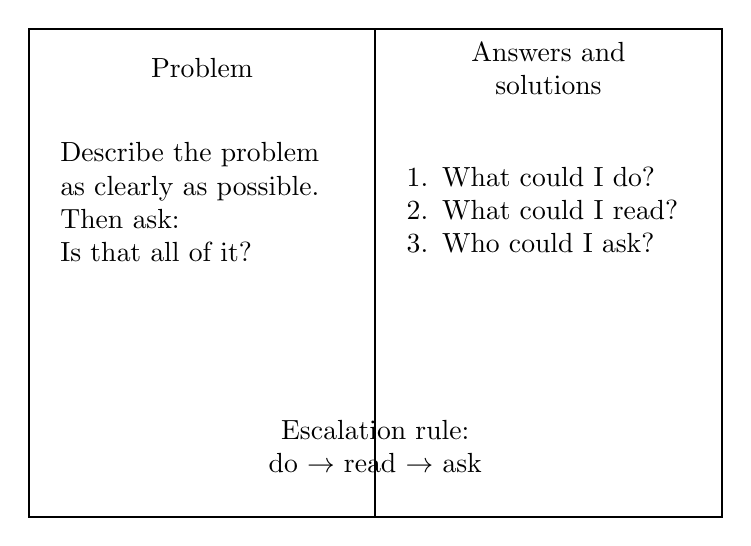
\begin{tikzpicture}[x=1cm,y=1cm]
\draw[thick] (0,0) rectangle (8.8,-6.2);
\draw[thick] (4.4,0) -- (4.4,-6.2);

\node[align=center] at (2.2,-0.5) {Problem};
\node[align=center] at (6.6,-0.5) {Answers and\\solutions};

\node[align=left,text width=3.6cm] at (2.2,-2.2) {Describe the problem\\as clearly as possible.\\Then ask:\\Is that all of it?};

\node[align=left,text width=3.6cm] at (6.6,-2.3) {1. What could I do?\\2. What could I read?\\3. Who could I ask?};

\node[align=center,text width=7.4cm] at (4.4,-5.3) {Escalation rule:\\do $\rightarrow$ read $\rightarrow$ ask};
\end{tikzpicture}
\caption{A transcript-backed page layout for the lecture's problem-solving method. The figure is an editorial reconstruction from spoken instructions rather than from board evidence.}
\end{figure}

The procedure can be written more explicitly:
\begin{align}
W_0(X) &= \text{state the problem } X \text{ as clearly as possible}, \\
W_1(X) &= \text{ask: Is that all of it?}, \\
U(X) &= \text{list what I could do}, \\
R_b(X) &= \text{list what I could read or research}, \\
A_s(X) &= \text{list who I could ask}.
\end{align}

The lecture then imposes a strict order:
\begin{equation}
\text{do} \rightarrow \text{read} \rightarrow \text{ask}.
\end{equation}

This order is one of the chapter's most important pieces of discipline. We do not ask first. We first try to solve the problem ourselves. If that fails, we search and research. If research still does not yield the answer, then we ask another person. Rohn even recycles the earlier search maxim here:
\begin{equation}
\text{search/research} \rightarrow \text{find}.
\end{equation}

The inner reason for postponing the third step is not pride but strength. If we borrow every answer too quickly, we fail to build the relevant powers:
\begin{align}
\text{trying first yourself} &\rightarrow \text{mental and emotional muscle}, \\
\text{helping yourself first} &\rightarrow \text{others respond more quickly with help}.
\end{align}

This is why Rohn recommends bringing working papers when we finally ask for help. A person who can say, ``I have tried this, I have read this, and I still do not see the answer,'' is easier to help and, more importantly, is already stronger. The attempt itself has developed discipline. The lecture's closing warning is implicit but firm: one day there may be no one else to ask.

\section{Summary}

The lecture begins with enlightened self-interest and ends with a sheet of working paper. Between those poles it builds one continuous argument. Need alone does not entitle us to a result. Qualification, sequence, and sustained action do. Planting precedes reaping. Knocking precedes open doors. Searching precedes finding. Asking precedes answers.

From there the law broadens. Seed matters more than disclosed need in the marketplace. Giving begins receiving. Service to many leads to greatness. Faithfulness with little prepares stewardship over much. Good ideas require good plans, and both require time. Patience is not passive resignation but the medium in which people, projects, and seasons ripen. Finally, when life becomes confused, we take the problem out of the head and put it on paper.

The chapter's mathematics remains modest, as it should. This is not a lecture in formal theory. It is a lecture about order, beginning, and sequence: what must come first, what can follow only afterward, and why durable results cannot be had by trying to skip the qualifying step.